
In the demonstration we run through a game of (a variant of) Hanabi. 
In Hanabi, each agent has cards with a color and a
number, but cannot see his/her own hand.
At each turn, in \emph{Hintikka's World}, the user can play the role of one of the agents: he/she can either give the information to some other agent about a number or a color, or play a card. The goal is to play the cards in increasing order for each color.
During the process, the system keeps track on the knowledge of the agents.
More precisely, the system shows the real world (the real distribution of the cards). When the user clicks an agent, the system displays a \emph{sampling} of some possible worlds for that agent (i.e., some distributions of cards he/she still considers as possible at this stage of the game). The agents also reason about knowledge of other agents, as shown in Figure~\ref{figure:guihanabi} (two levels of knowledge are shown).
%
%
%% expliquer la démo. Je me suis peut etre trompé sur le nombre de cartes ici et si on gère les jetons pour les infos il faut le mettre dans le paragraphe.
% Alex: pas grave au pire. on dit qu'on peut faire ça ou ça, c'est pas _forcément_ exclusif.
%


\begin{figure}
	\begin{center}
		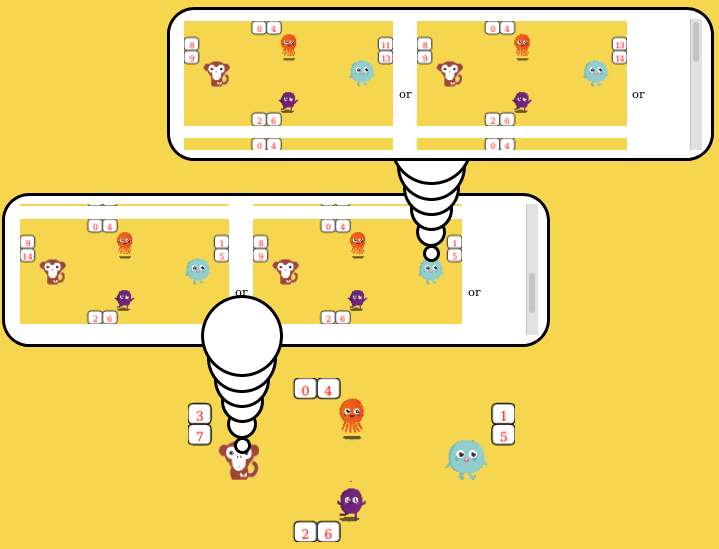
\includegraphics[width=4cm]{images/HW_screenshot_hanabi.png}
	\end{center}
\vspace{-3mm}
	\caption{Screenshot of Hanabi in \emph{Hintikka's World}.\label{figure:guihanabi}}
\end{figure}
%%\newpage

Note that in this demonstration, in order to explain models of DEL, the tool still presents examples that rely on explicit models, such as ``Sally and Anne'', ``Muddy Children'', ``Consecutive Numbers'', etc.
